\section*{Quasi-Steady-State Simulation}

\begin{frame}{Quasi-Steady-State Simulation}
    \begin{columns}
        \column{0.5\textwidth}
        \begin{itemize}
            \item The track is broken down into a mesh of discrete time or distance steps (similar to finite element analysis)
            \item Acceleration is assumed to be constant at each step
            \item The finer the mesh, the more accurate the result
        \end{itemize}
        \column{0.5\textwidth}
        \centering
        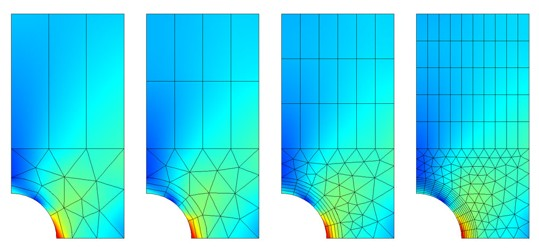
\includegraphics[width=\textwidth]{res/Finite Element Mesh.jpg} \\
        \textit{Finite Element Mesh} \\
        \vspace{2ex}
        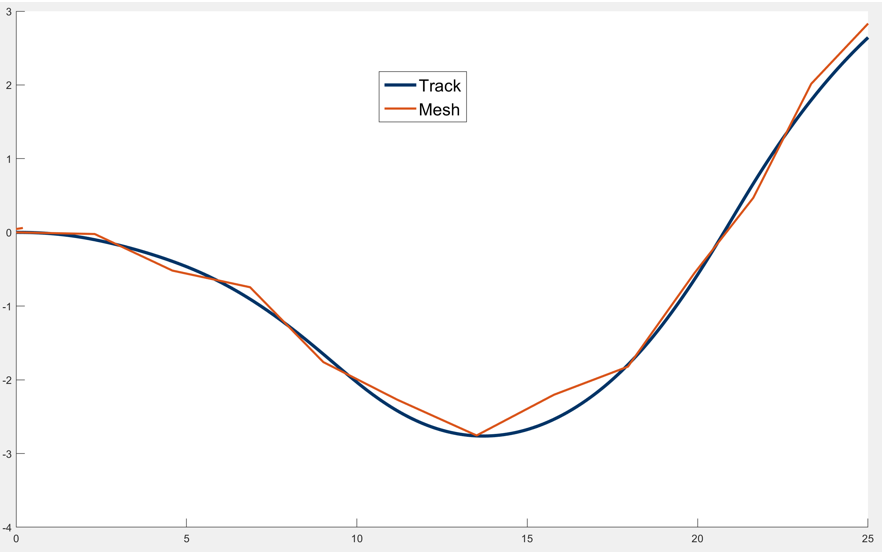
\includegraphics[width=\textwidth]{res/Track Mesh.png} \\
        \textit{Track Mesh}
    \end{columns}
\end{frame}

\begin{frame}{Track Mesh}
    The shape, elevation, banking, and grip factor of the track
    is defined in a spreadsheet.
    This is converted to a mesh with approximately equal distance steps.
    \begin{columns}
        \column{0.4\textwidth}
        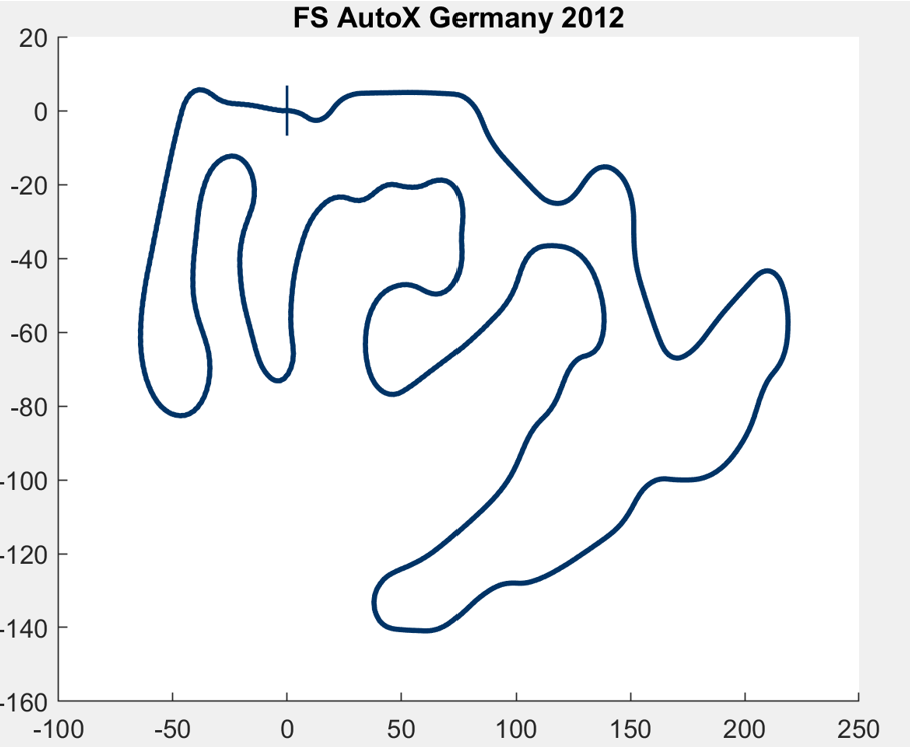
\includegraphics[width=\textwidth]{res/Track Diagram.png} \\
        \column{0.6\textwidth}
        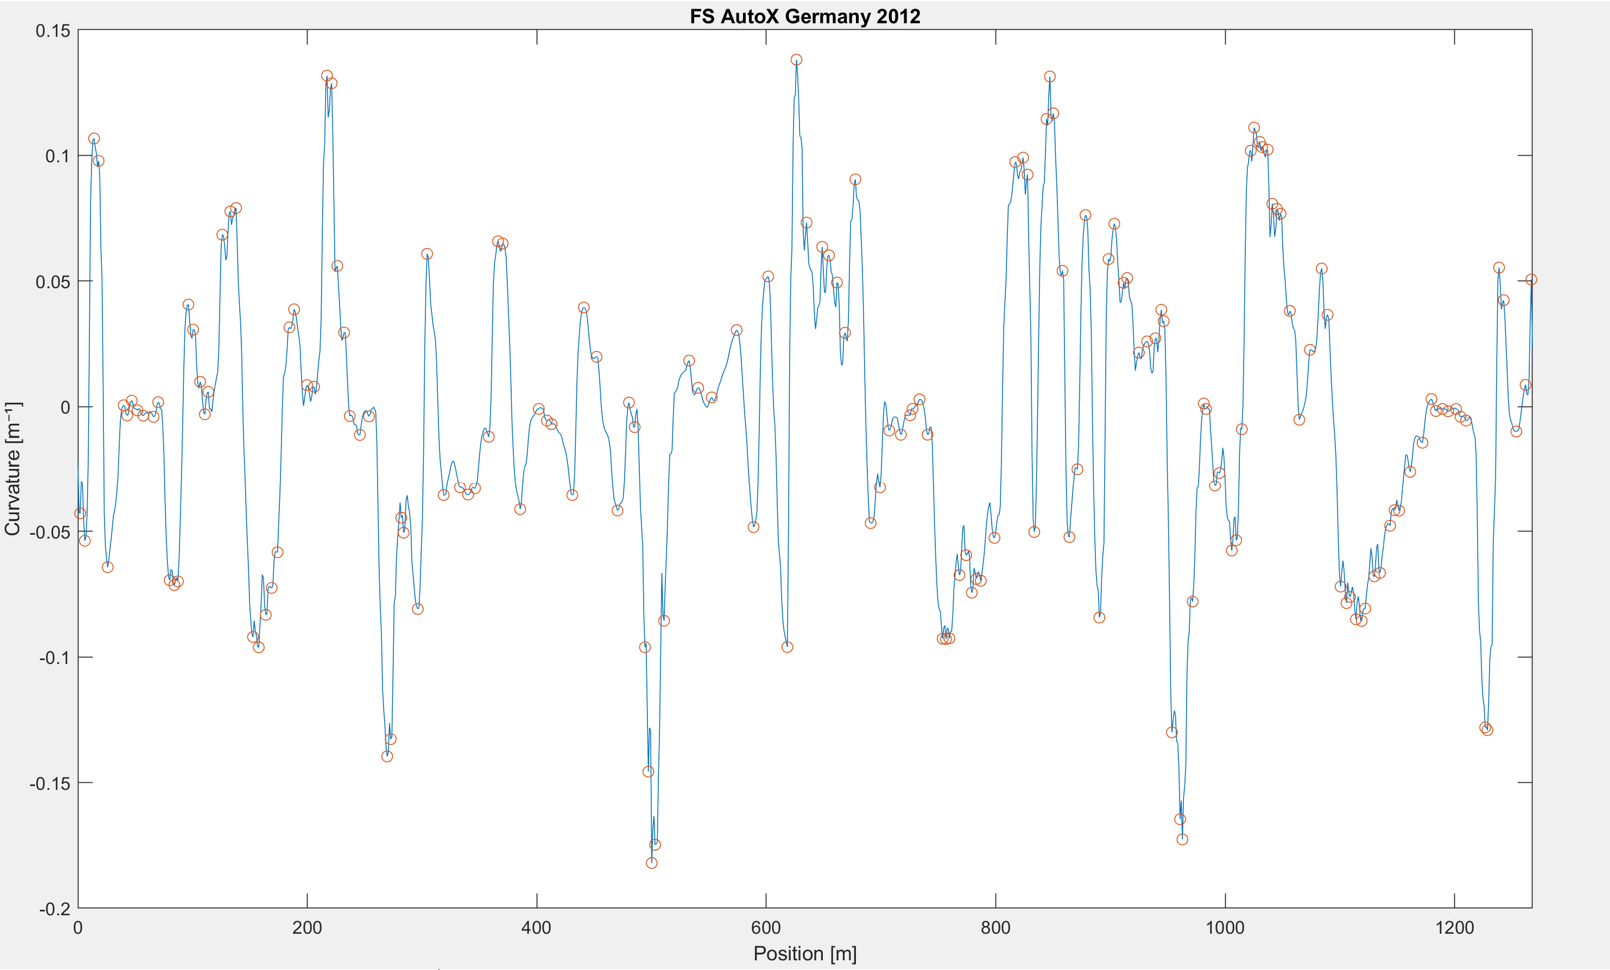
\includegraphics[width=\textwidth]{res/Mesh Curvature.png}
    \end{columns}
    Apexes are identified as the points where curvature is at a maximum.
\end{frame}

\begin{frame}{QSS Solver Process}
    Aero forces and load transfer are affected by velocity and acceleration.
    Therefore, an iterative process is required.
    \vspace{2ex}
    \begin{columns}
        \column{0.22\textwidth}
        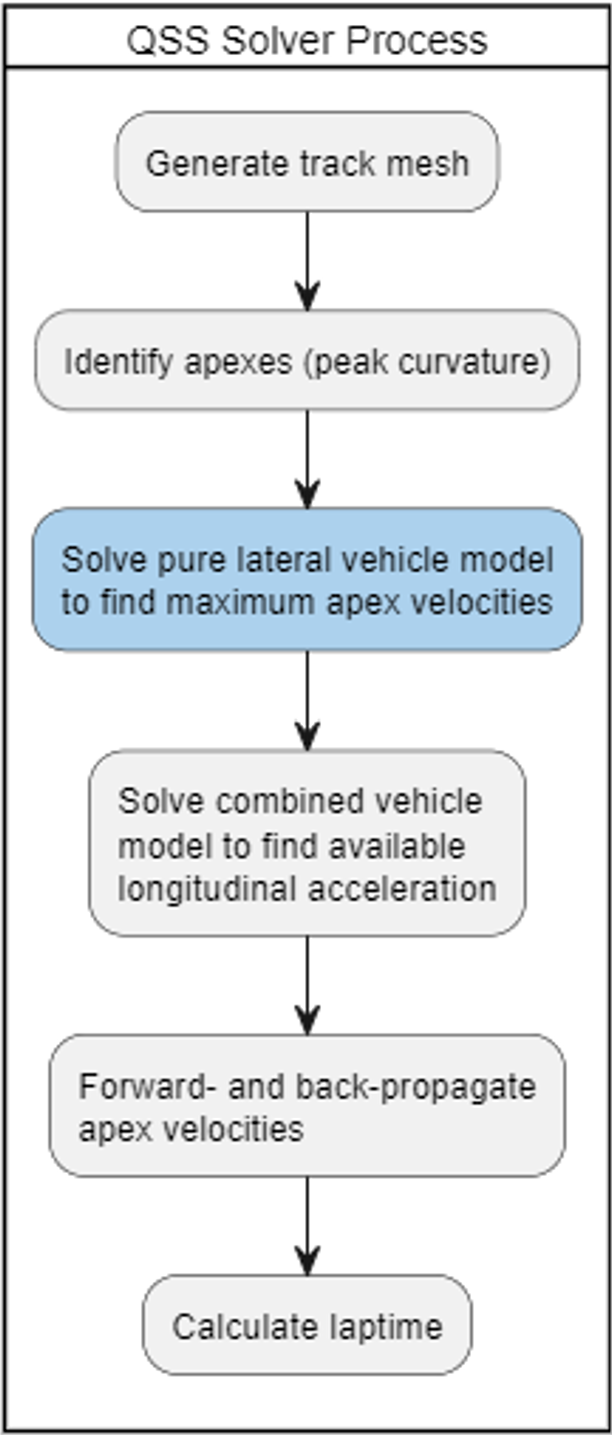
\includegraphics[width=\textwidth]{res/QSS Solver Process.png} \\
        \column{0.65\textwidth}
        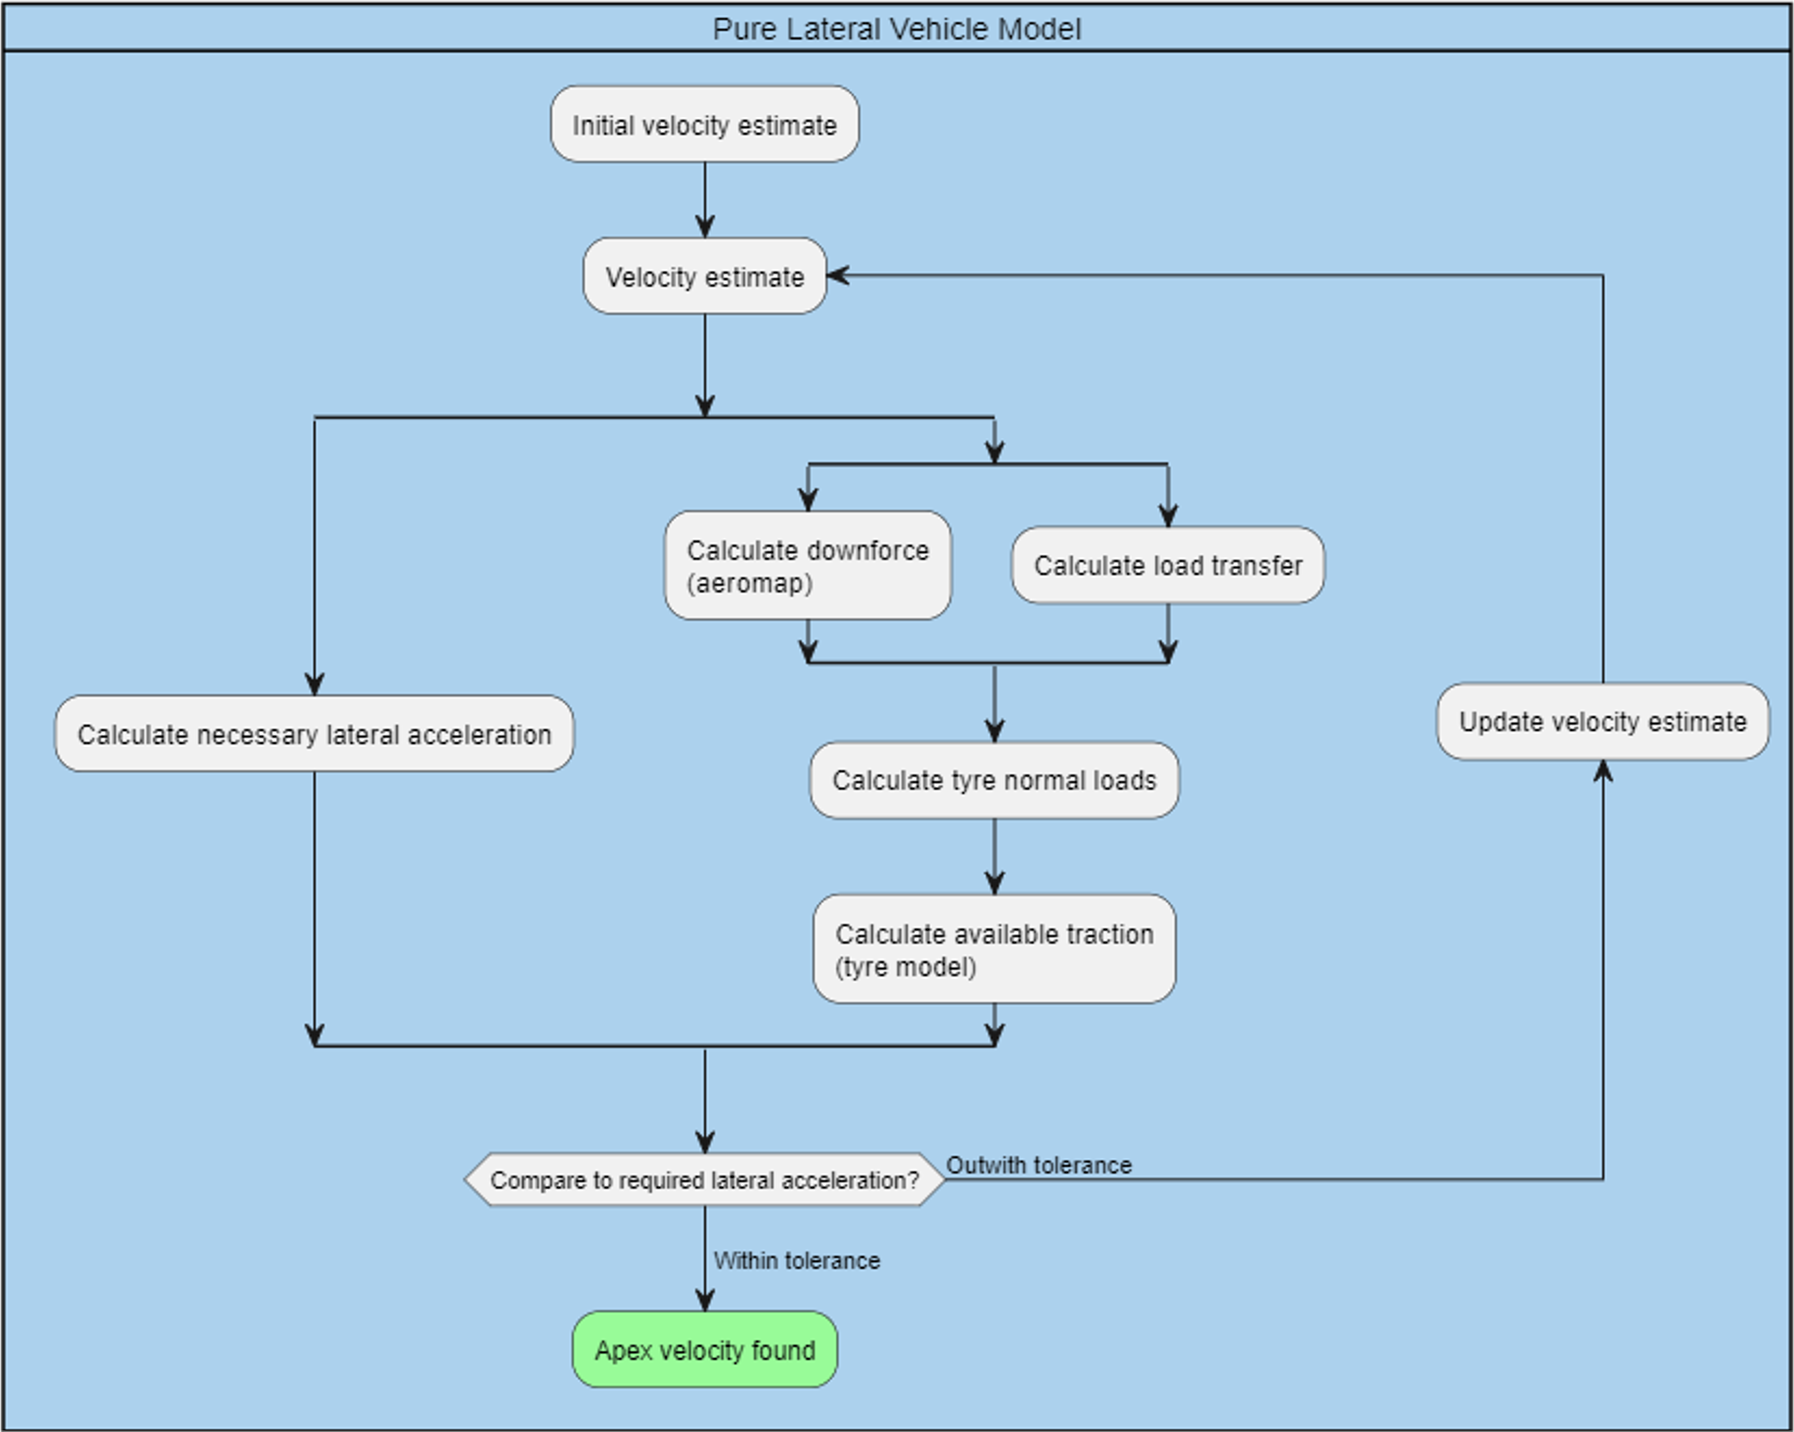
\includegraphics[width=\textwidth]{res/Lateral Vehicle Model.png} \\
    \end{columns}
\end{frame}